\section{Creating a local repository\label{sec:local_repo}}

This section will cover the following points

\begin{enumerate}
	\item Registering a github username
	\item Download git software
	\item Fork the master repository
\end{enumerate}

\subsection{Git Username and Profile}

The first step is to create a username and profile on github (if you do not already have one). Creating a username and profile on github is free and easy to do. 

Go to \url{https://www,github.com} to register a username and set up a profile if you do not already have one. See the help at github for more information. Once you have set up a github account you need download the git software that you use to ``communicate" with repositories (places where the software source code is stored) on github.

\subsection{Git Software}

You will need to acquire a git client in order to clone a copy of the source code and link this to the repository.

\CNAME\ also requires a command line version of git in order to compile. The \CNAME\ build environment requires git in order to evaluate the version of the code used at compile time to include into the executable and manual when being built. 

One package that allows this on a Microsoft Windows platform is tortoisegit (see \url{https://tortoisegit.org/download}) to pull, push and commit changes to git repositories. However there are many other clients that could be used to achieve the same functionality.

\subsection{Cloning a repository}

The publicly available \CNAME\ code is in the master repository. Only the \CNAME\ Development Team have permission to add, delete, or change code in the master repository. Other contributors can either add, delete, or change code either by forking the master repository' or by maintaining a local version of the repository. Forking a copy on github can be done at \url{https://github.com/NIWAFisheriesModelling/CASAL2} by selecting the fork button in the top right of the page circled in Figure~\ref{fig:fork}

\begin{figure}[!ht]
	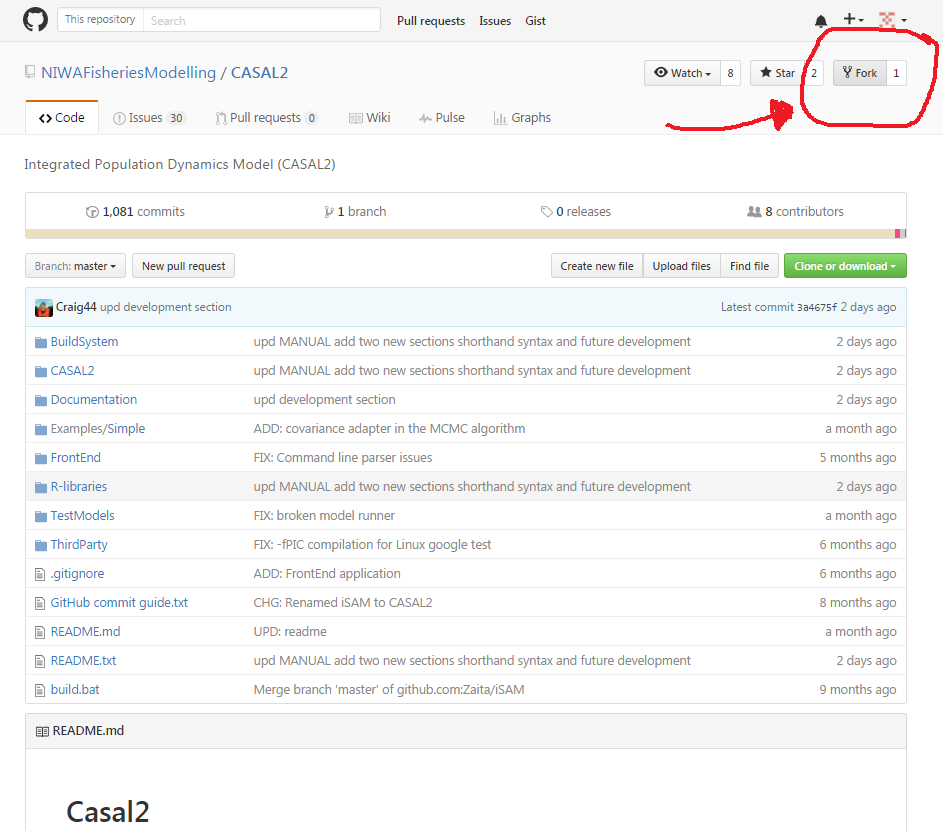
\includegraphics[scale=0.6]{Figures/Fork_button.png}
	\caption{Creating a forked repository}\label{fig:fork}
\end{figure}
\pagebreak

This will create a copy of the \CNAME\ repository under your profile at the point of the fork. To check that you have successfully forked the repository, go to your git profile and you should see a \CNAME\ repository under your repositories, shown in Figure~\ref{fig:fork_success},

\begin{figure}[!ht]
	\includegraphics[scale=0.6]{Figures/Fork_success.png}
	\caption{Fork success}\label{fig:fork_success}
\end{figure}

An important point is that the forked repository will not automatically keep up to date with the master repository. So if the master changes, you will want to keep your forked repository up to date. This can easily be done and is explained in the next section.


